\documentclass[a4j,10pt, twocolumn]{jarticle} \usepackage[dvipdfmx]{graphicx} \usepackage{amssymb} \usepackage{amsmath}
\usepackage{float}
\usepackage{slashbox}
\usepackage[compact]{titlesec}
%---------------------------------------------------
% ページの設定
%---------------------------------------------------
\setlength{\textwidth}{179truemm}
\setlength{\textheight}{263truemm}
\setlength{\topmargin}{-12.5truemm}
\setlength{\oddsidemargin}{-9.5truemm}
\pagestyle{empty}
\setlength{\headheight}{-2truemm}
\setlength{\parindent}{1zw}

\begin{document}
\twocolumn
[
\begin{center}
  {\huge NAISTにて取り組みたい研究について}
\end{center}
\begin{flushright}
\begin{tabular}{ll}
氏名: & 新妻巧朗\\
試験区分: & 情報科学区分\\
希望研究室: & 自然言語処理研究室
\end{tabular}
\end{flushright}
\vspace{1truemm}
]
\section{はじめに}
\subsection{NAISTで取り組みたいこと}
NAISTにて、私が取り組みたい研究テーマは「情報検索システムにおけるファセットの自動生成手法」である。

このファセットとは、図書館情報学の「あるクラスを2以上の異なる区分特性によって区分したときに得られる下位クラスの総体\cite{libdic}」という定義を指す。
また、この区分特性は「ある分類に属する個々のメンバーに共通する性質」のことを言う。
そして、ファセットを具体的に説明すると、共通の性質を抽出することで得られたある区分で検索結果を絞り込む切り口のことである。
\section{研究の概要}
\subsection{背景・社会的意義}
 現代社会において情報収集をするためには、検索エンジンを利用することは必要不可欠である。
 しかし、検索エンジンを適切に活用できず、目的の情報に至れない場面も多い。
 それは多くの検索エンジンの仕組みが、利用者に対して情報検索能力を要求しているからである。
 これまでも福島らの研究によって情報検索能力は個人差が大きく、能力差によって情報格差が生じていることが調査されてきた\cite{fukushima}。
 こうした課題を解決することで、情報に辿りつけないために生じる機会損失を減らすことができるのではないかと考えている。
 過去に齋藤らによる教育を通して情報検索能力を向上させる研究\cite{saito}も存在しているが、本研究ではシステムの拡張によって解決するアプローチを考えていく。

 福島らによって言語能力の高さが情報検索能力の高さに関係しているとわかった\cite{fukushima}。
 つまり、言語能力の高低が情報検索において、情報格差を生み出していると考えられる。
 そのため、情報の探索過程の言語能力を要求する場面で利用者の補助をおこなうシステムを提案したい。
\subsection{提案内容}

 そこで、入力された検索質問に対して適切なファセットを表示し選択させることで、検索質問を検索意図に近づけていくシステム(図1)を提案したい。

 \begin{figure}[ht]
   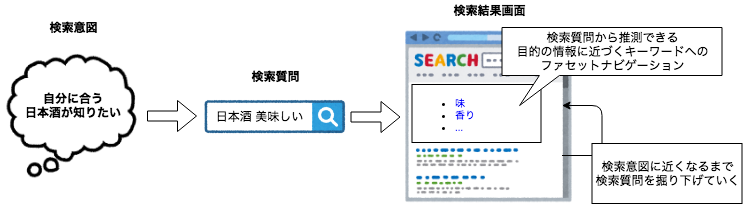
\includegraphics[width=85mm]{./new_ir_with_navi.png}
   \caption{システムのイメージ図}
 \end{figure}
 
 検索意図とは、人が検索行動をおこなう動機のことである。
 情報の探索行動は、検索質問を検索の動機を満たす文書に近づけるプロセスであると考えられる。
 そのため、ファセット検索が利用できるのではないかと考えた。
 ファセット検索とは、検索システムの利用者に検索対象を何らかの区分で絞り込むファセットを選択させ、検索対象を絞り込む検索手法である\cite{faceted}。
 これはシステムの利用者が検索意図を言語化する行動をシステムが代行していると言える。
 そのため、検索エンジンが個人の言語能力に依存している問題にアプローチできると考えている。
\section{研究の方法}
\subsection{従来のファセット検索の課題}
 ファセット検索の典型的な用例として、Amazon.co.jp\cite{amazon}の検索結果画面をあげる。
 ファセット検索は図2の赤枠で囲われたメニューのように、ある分類に関する検索結果をさらに絞り込む選択肢を提供する。
 \begin{figure}[ht]
   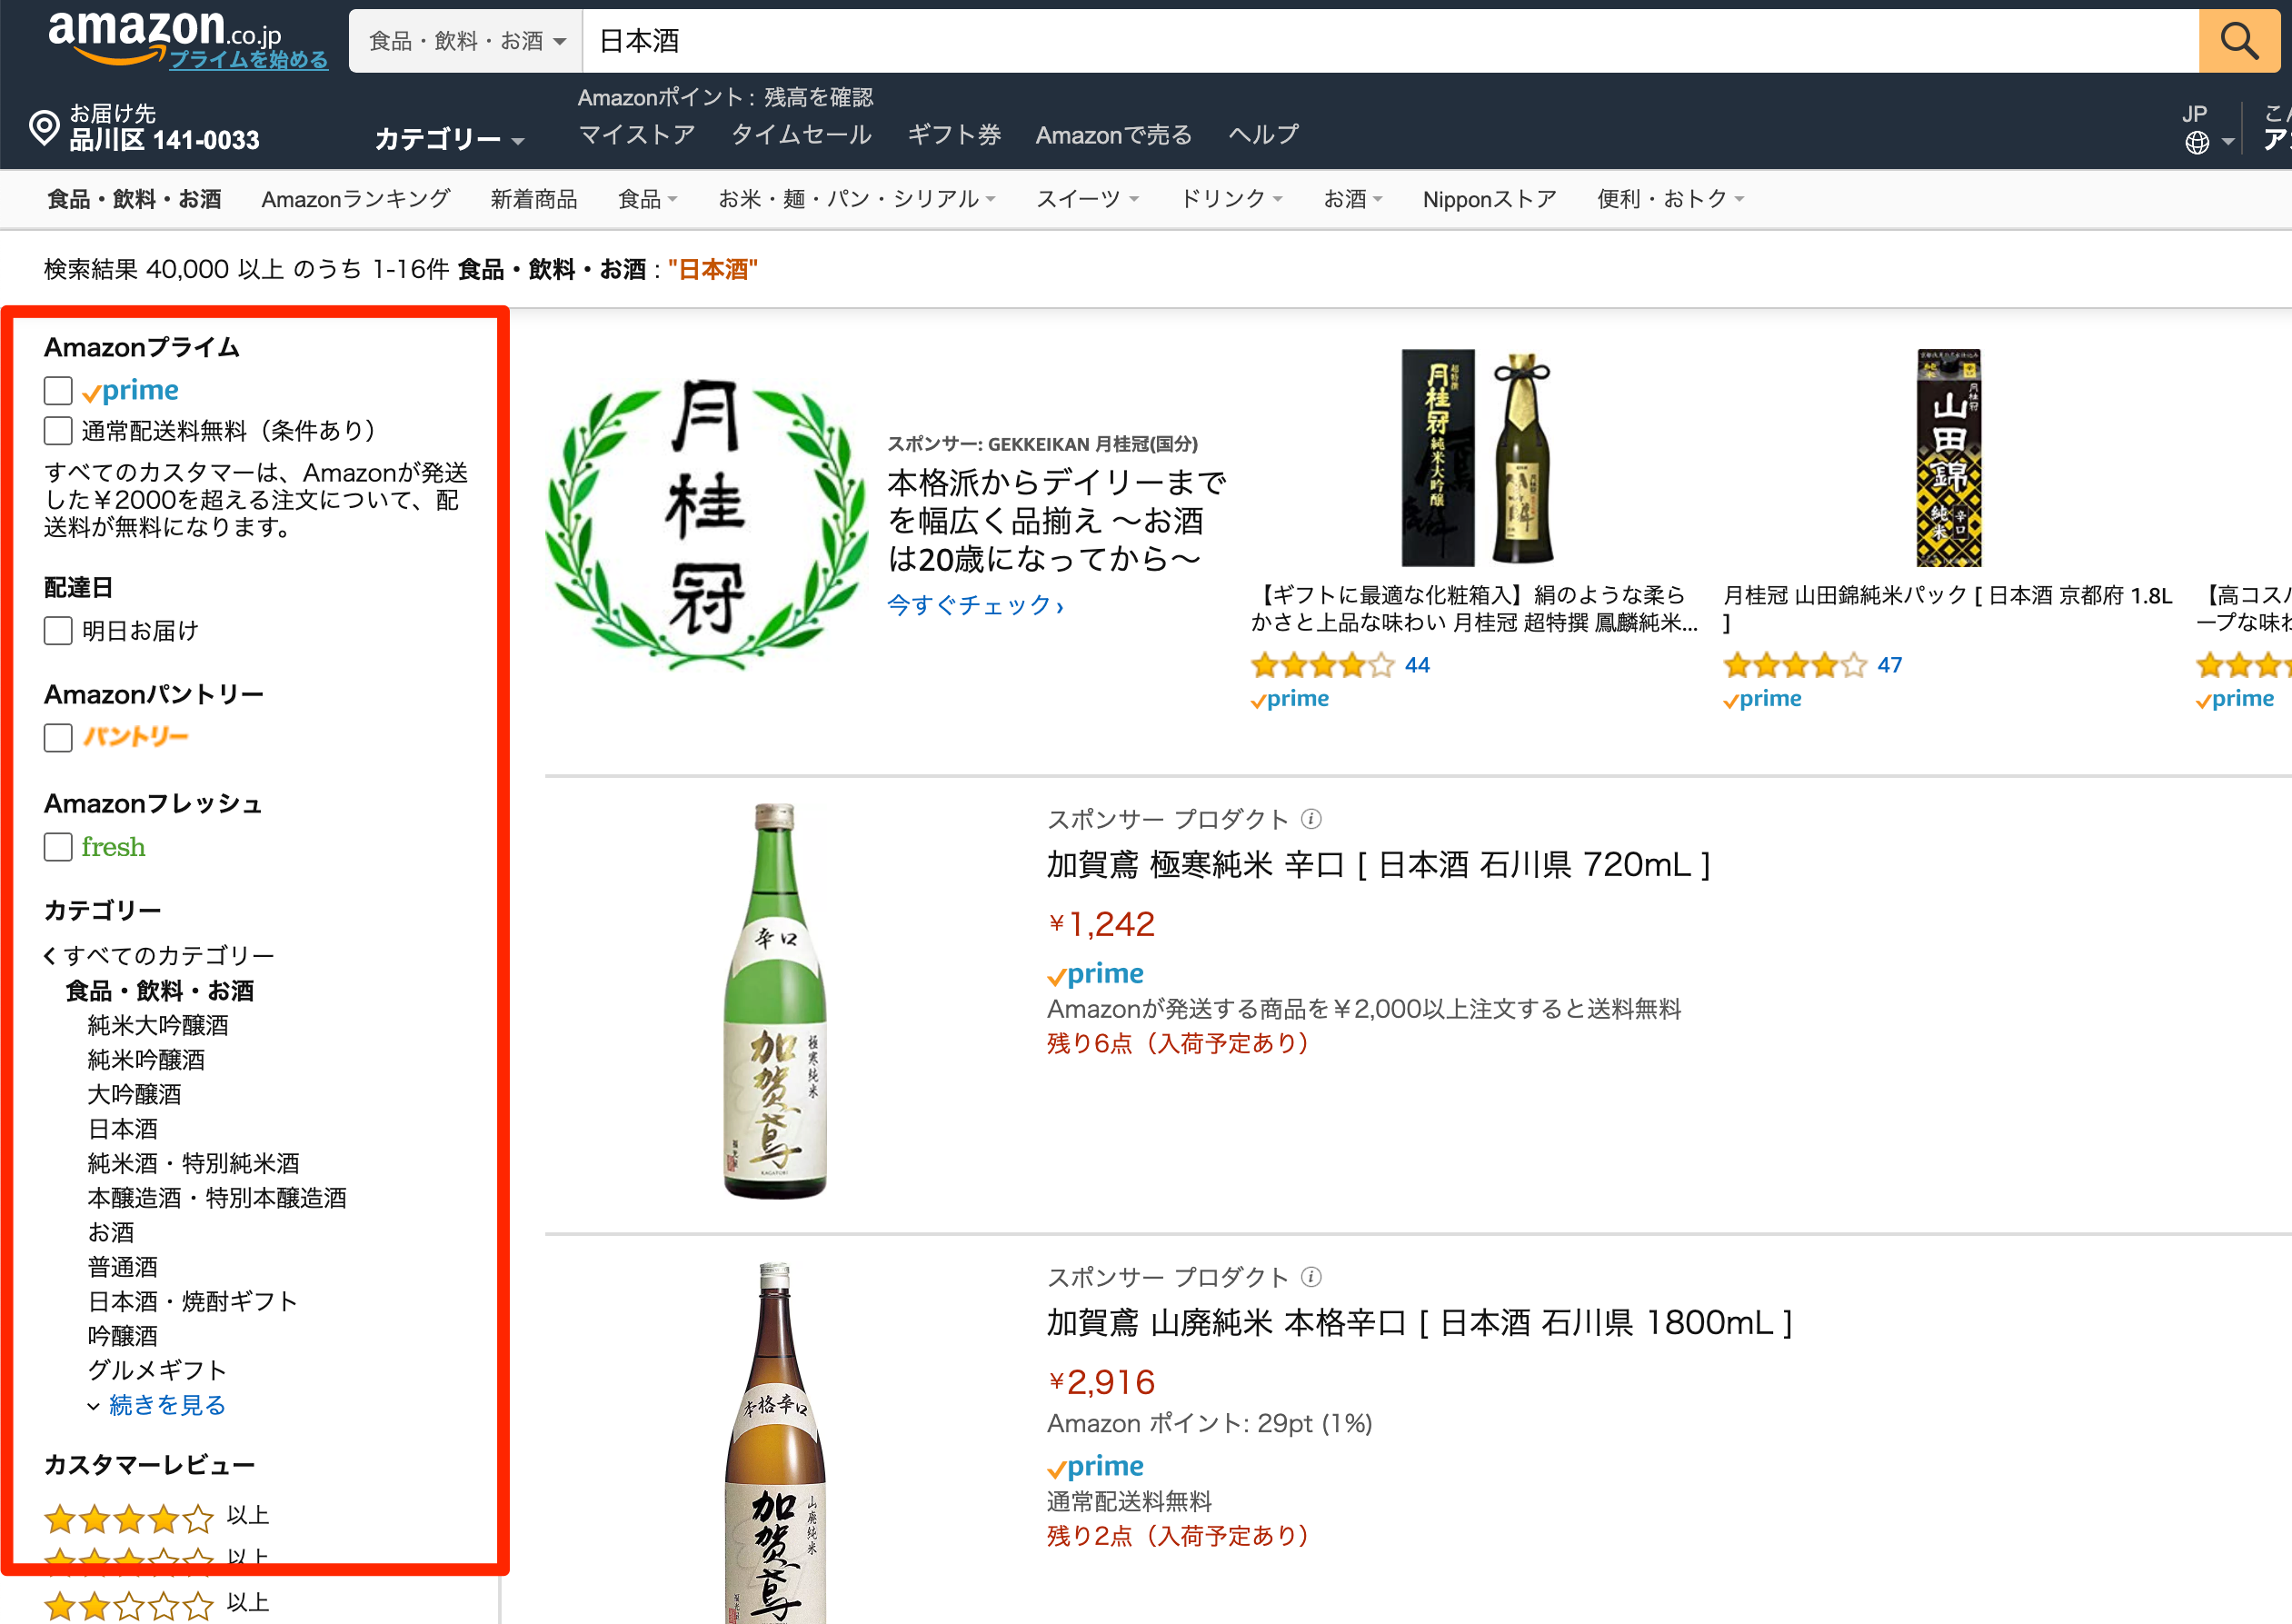
\includegraphics[width=85mm]{./amazon.png}
   \caption{Amazonの検索結果画面: 日本酒に対するファセット検索}
 \end{figure}
 この例では、商品データを検索対象として索引している。このように従来のファセット検索では、検索対象になる文書には既に構造化がなされ、属性データを持っているものを利用することが多い。
 この属性データとは、ある区分特性に属しているかどうかを示すメタデータのことである。
 また、ファセット検索を非構造的な文書に利用する場合には、ファセットを作成しその情報をメタデータとして追加して半構造的な文書にする。
 そのためには、事前に文書から区分特性を見つけ出して索引可能な属性データに変換し、文書に付与する必要がある。
 従来であれば、この作業は人手を用いておこなわれてきた。
 しかし、Webを対象にファセットを作成する場合には、文書の増減と文書分類の変化が早く人手による作業が現実的でないという課題がある。
 そこで区分特性を推測し自動的に属性データを付与することで、ファセット検索をWebにも応用できるようにしたいと考えた。

\subsection{研究の方向性}
本システムではファセットを作成するために必要な二つのデータを出力をすることを目標とする。
\begin{description}
  \item[ファセットを表すtupleのリスト] ある語彙$v$を上位クラスとして、$v$がある区分特性$c$を介して関係する語彙の集合$V$を下位クラスとして考えるとき、それらのデータからなる$\langle v, c, V\rangle$形式のtupleのリスト。
  \item[属性データ] 文書があるファセットに含まれるかどうかを示すデータ。文書に付与するメタデータとして考える。
\end{description}

\subsubsection{ファセットを表すtupleのリスト}
索引する文書を入力データとしたときの、このtupleの情報を抽出する方法を考える。
本システムにおいて、区分特性には述語を活用することを提案したい。
述語は「主語について、その動作・作用・性質・状態などを叙述するもの」と定義されている\cite{daijisen}。
そのため、述語は主語にとって目的語がどんな操作対象、性質、状態かを表すと考えられ、主語と目的語の関係を表す語と見なせるからだ。

ここで、区分特性の抽出にはOpenIEと呼ばれる研究の成果を活用できる可能性がある。
OpenIEは文章から$\langle \arg1, rel, \arg2 \rangle$形式のtupleで、情報を抽出をする研究分野である\cite{niklaus}。
文書中の述語をrelとして、その周辺の語彙などをarg1, arg2として抽出する。
このとき、arg1を語彙$v$、relを区分特性$c$とみなせば、arg1とrelが一致しているtupleをまとめ、それぞれのarg2を集めて下位クラスの語彙の集合$V$にすることで、$\langle v, c, V\rangle$のtupleを作成できると考えている。

例えば、「日本酒」を語彙$v$とすると、区分特性$c$は「の銘柄は」といった述語となる。そして、その目的語である「一ノ蔵」「花浴陽」などをまとめて語彙の集合$V$を得れば、$\langle "日本酒", "の銘柄は", ["一ノ蔵", "花浴陽", \dots] \rangle$というtupleを作れる。

\subsubsection{属性データ}
 3.2.1にて作成したtupleの上位クラスである語彙$v$を使う。語彙$v$が文書に関係しているかをブール値で表現し、メタデータとして付与することで実現する。tf-idfなどに閾値をもうけて関係性を表現することを検討している。
\subsubsection{まとめ}
 ユーザインタフェースを作成するのに3.2.1のtupleを利用する。例えば、検索質問の語彙と3.2.1のtupleの語彙$v$が一致するファセットを検索結果画面に表示する。そして、検索処理では3.2.2で文書に付与した属性データを利用することで、提案をしたシステムが実現できるのではないかと考えている。

\section{これまでの修学経験等}
 学部では地方の産業構造に関する実証分析をする研究してきた。
 特に卒業研究では総生産と地域を構成する産業に目をつけ、経済格差が生じる要因について分析をした。
 また、社会人ではWebサービスにソフトウェアエンジニアとして携わり、検索システムの利用者が得たい情報をどう探索しているかについて考えてきた。
 特に現在携わっているアルバイト求人のデータベースメディアでは、どうファセットナビゲーションを実現するとよいのか、求人検索機能のファセット検索をどう実装すべきかなどを試行錯誤する機会に恵まれた。
 こうした経験が本研究では役立つのではないかと考えている。

\section{最後に}
ここまでNAISTにて取り組みたい研究テーマや自身の経験について述べてきた。
私がNAISTを志望するのは、様々な経歴を持った人間を受け入れ、かつそのサポート体制が整っており優れた研究成果を出している大学院であるからだ。
こうしたNAISTの整った教育・研究環境を活かして、自然言語処理や情報検索の分野に貢献していきたい。

\begin{thebibliography}{9}
\bibitem{libdic}
  日本図書館情報学会用語辞典編集委員会編 (2013), 図書館情報学用語辞典 第4版
\bibitem{fukushima}
   福島健介・小原 格・須原慎太郎・ほか (2005), インターネット検索能力の差異に及ぼす 要因の検討 その1, コンピュータ&エデュケーション VOL.18 2005
\bibitem{saito}
   齋藤ひとみ・三輪和久 (2004),  Web 情報検索におけるリフレクションの支援, 人工知能学会論文誌 19 巻 4 号 C (2004 年)
\bibitem{faceted}
  Daniel Tunkelang (2009), Faceted Search (Synthesis Lectures on Information Concepts, Retrieval, and Services), pp. 21―26
\bibitem{amazon}
  Amazon.co.jp (2019/5/23), https://www.amazon.co.jp/
\bibitem{daijisen}
  池上秋彦・金田弘・杉崎一雄・ほか (2019/4), デジタル大辞泉
\bibitem{niklaus}
  Christina Niklaus, Matthias Cetto, Andre Freitas, and Siegfried Handschu (2018), A Survey on Open Information Extraction, Proceedings of the 27th International Conference on Computational Linguistics
\end{thebibliography}
\end{document}
